
%%%%%%%%%%%%%%%%%%%%%%%%%%%%%%%%%%%%%%%%%%%%%%%%%%%%%%%%%%%%%%%%%%%%%%%%%%%%%%
\section{Definici�n}
\begin{frame}
\frametitle{Introducci�n}
\begin{block}

Sea \textcolor{blue}{$n$} un entero positivo. Una \textit{\textcolor{blue}{sucesi�n arb�rea}} es una sucesi�n de enteros positivos \textcolor{blue}{ $d_1, d_2,\ldots d_n$} tal que \textcolor{blue}{ $\sum_{1\le i\le n} d_i=2(n-1)$}.
\end{block}
 
\begin{block}

Una sucesi�n \textcolor{blue}{ $\sigma= d_1, d_2,\ldots d_n$} es arb�rea si y solo si hay un �rbol cuyos v�rtices tienen grados \textcolor{blue}{ $d_1, d_2,\ldots d_n$}.
\end{block}
\end{frame}

\begin{frame}
\begin{figure}[!ht]
\begin{center}
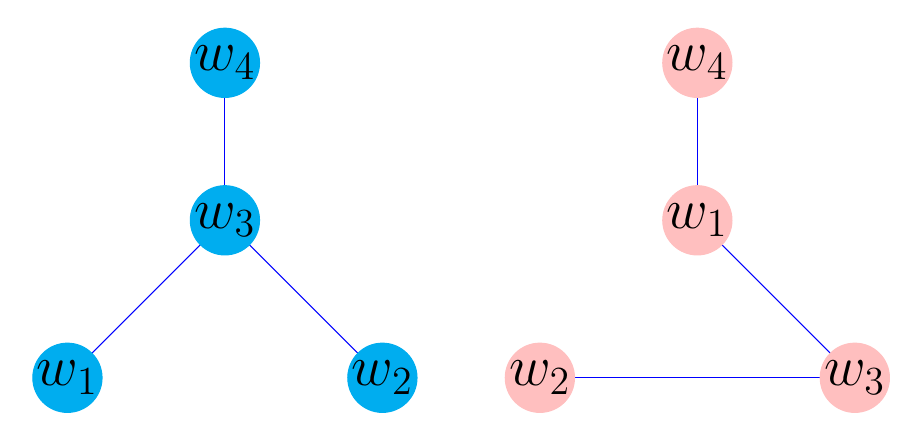
\begin{tikzpicture}[scale=0.5]

\draw[-,color=blue] (4,8) to  (4,4);
\draw[-,color=blue] (0,0) to (4,4);
\draw[-,color=blue] (8,0) to (4,4);


\filldraw[color=cyan] (0,0) circle (25pt) node[]{\huge \textcolor{black}{$w_1$}};
\filldraw[color=cyan] (8,0) circle (25pt) node[] {\huge \textcolor{black}{$w_2$}};
\filldraw[color=cyan] (4,4) circle (25pt) node[] {\huge \textcolor{black}{$w_3$}};
\filldraw[color=cyan] (4,8) circle (25pt) node[] {\huge \textcolor{black}{$w_4$}};

%%%%%%%%%%%%%%%%%%%%%%%%%%%%%%%%%%%%%%%%%%%%
\draw[-,color=blue] (16,8) to  (16,4);
\draw[-,color=blue] (12,0) to (20,0);
\draw[-,color=blue] (20,0) to (16,4);


\filldraw[color=pink] (16,8) circle (25pt) node[]{\huge \textcolor{black}{$w_4$}};
\filldraw[color=pink] (12,0) circle (25pt) node[] {\huge \textcolor{black}{$w_2$}};
\filldraw[color=pink] (20,0) circle (25pt) node[] {\huge \textcolor{black}{$w_3$}};
\filldraw[color=pink] (16,4) circle (25pt) node[] {\huge \textcolor{black}{$w_1$}};

\end{tikzpicture}
\end{center}
\end{figure}
\hspace{1.5 cm } $\sigma=1,1,3,1$ \hspace{4cm} $\sigma= 2,1,2,1$

\end{frame}
%%%%%%%%%%%%%%%%%%%%%%%%%%%%%%%%%%%%%%
%\begin{frame}
%\begin{figure}[!ht]
%\begin{center}
%\begin{tikzpicture}[scale=0.7]
%\draw[-,color=blue] (4,8) to  (4,4);
%\draw[-,color=blue] (0,0) to (4,4);
%\draw[-,color=blue] (8,0) to (4,4);
%
%
%\filldraw[color=orange] (0,0) circle (25pt) node[]{\huge \textcolor{black}{$w_1$}};
%\filldraw[color=orange] (8,0) circle (25pt) node[] {\huge \textcolor{black}{$w_2$}};
%\filldraw[color=orange] (4,4) circle (25pt) node[] {\huge \textcolor{black}{$w_4$}};
%\filldraw[color=orange] (4,8) circle (25pt) node[] {\huge \textcolor{black}{$w_3$}};
%\end{tikzpicture}
%\end{center}
%\end{figure}
%\centering $\sigma=1,1,1,3$ 
%\end{frame}
%





%%%%%%%%%%%%%%%%%%%%%%%%%%
\section{Objetivo de la pl�tica}
\begin{frame}
\frametitle{Objetivo de la pl�tica }
\begin{thm}
%\frametitle{Objetivo de la pl�tica }
Sean \textcolor{blue}{$n\geq 4$} un n�mero entero, \textcolor{blue}{$G$} una gr�fica etiquetada con el conjunto de v�rtices \textcolor{blue}{ $V(G)= \left\lbrace w_1, w_2, \ldots, w_n \right\rbrace$} y \textcolor{blue}{$\sigma=d_1, d_2 \ldots, d_n$} una sucesi�n de grados arb�rea, donde  \textcolor{blue}{$d_1 \leq d_2 \leq \cdots \leq d_n$}. El problema de decidir si \textcolor{blue}{$G$} tiene un �rbol generador \textcolor{blue}{ $T$} tal que \textcolor{blue}{$d_T(w_i)=d_i$}, con \textcolor{blue} {$1 \leq i \leq n $}, es \textcolor{blue}{$NP$-completo}. 
\end{thm}
\pause
%\begin{frame}
\begin{figure}[!ht]
\begin{center}
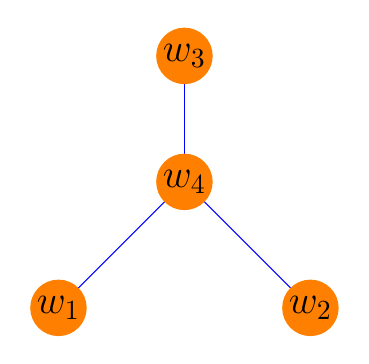
\begin{tikzpicture}[scale=0.4]
\draw[-,color=blue] (4,8) to  (4,4);
\draw[-,color=blue] (0,0) to (4,4);
\draw[-,color=blue] (8,0) to (4,4);


\filldraw[color=orange] (0,0) circle (25pt) node[]{\Large \textcolor{black}{$w_1$}};
\filldraw[color=orange] (8,0) circle (25pt) node[] {\Large \textcolor{black}{$w_2$}};
\filldraw[color=orange] (4,4) circle (25pt) node[] {\Large \textcolor{black}{$w_4$}};
\filldraw[color=orange] (4,8) circle (25pt) node[] {\Large \textcolor{black}{$w_3$}};
\end{tikzpicture}
\end{center}
\end{figure}
\centering $\sigma=1,1,1,3$ 
%\end{frame}
\end{frame}

%%%%%%%%%%%%%%%%%%%%%%%%%%%%%%%%%%%%%%%%%%%%%%%5z
\section{Estrategia}
\begin{frame}
\frametitle{Estrategia usual}


\begin{itemize}
 \Large
\centering \item Mostrar que el problema de decisi�n \textcolor{blue}{$B$} esta \

en la \textcolor{blue}{clase $NP$}\pause
\vspace{1.5 cm}
\centering \item  $A\leq _ {\textcolor{blue}{p}} B$

\end{itemize}

\end{frame}
%%%%%%%%%%%%%%%%%%%%%%%%%%%%%%%%%%%%%%%%%%%%%%%%%%%%%%%%%%%%%%%%%%%%


\section{Estrategia.}
\begin{frame}
\frametitle{Estrategia usual.Punto n�mero uno}

%\begin{center}
\begin{itemize}
 \Large
\centering \item Mostrar que el problema esta en la clase $NP$ 



\end{itemize}
%\end{center}
\end{frame}
%%%%%%%%%%%%%%%%%%%%%%%%%%%%%%%%%%%%%%%%%%%%%%%%%%%%%%%%%%%%%%%
\section{Estrategia}
\begin{frame}
\frametitle{Estrategia usual. Punto n�mero dos}
\begin{itemize}
\centering \item $A\leq _p B$
\end{itemize}
%%%%%%%%%%%%%%%%%%%%%%%%%figura%%%%%%%%%%%%%%%%%%%%%%%%%%%%%%555
\begin{figure}[!ht]
\begin{center}
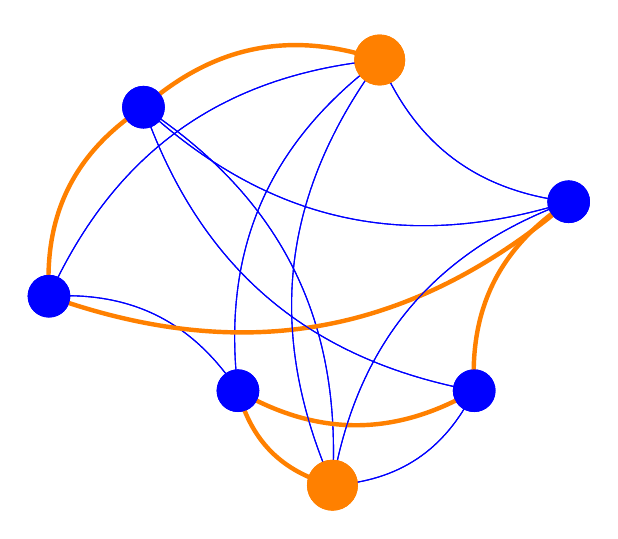
\begin{tikzpicture}[scale=0.3]

\draw[-,color=blue] (14,2) to [bend left] (10,6);
\draw[-,color=blue] (14,2) to [bend right] (20,6);
\draw[-,color=blue] (10,6) to [bend right] (2,10);
\draw[-, color=blue] (2,10) to [bend left] (6,18);
\draw[-, color=blue] (20,6) to [bend left] (24,14);
\draw[-, color=blue] (6,18) to [bend left] (16,20);
\draw[-,color=blue] (16,20) to [bend right] (24,14);

\draw[-,color=blue] (16,20) to [bend right] (2,10);
\draw[-,color=blue] (16,20) to [bend right] (10,6);
\draw[-,color=blue] (6,18) to [bend left] (14,2);
\draw[-, color=blue] (2,10) to [bend right] (24,14);
\draw[-, color=blue] (10,6) to [bend right] (20,6);
\draw[-,color=blue] (24,14) to [bend right] (14,2);
\draw[-,color=blue] (16,20) to [bend right] (14,2);
\draw[-,color=blue] (6,18) to [bend right] (20,6);
\draw[-,color=blue] (6,18) to [bend right] (24,14);
\draw[-, color=blue] (10,6) to [bend right] (14,2);

\filldraw[color=orange] (14,2) circle (30pt);
\filldraw[color=blue] (10,6) circle (25pt);
 \filldraw[color=blue] (20,6) circle (25pt);
 \filldraw[color=blue] (2,10) circle (25pt); 
 \filldraw[color=blue] (6,18) circle (25pt);
 \filldraw[color=blue] (24,14) circle (25pt);
\filldraw[color=orange] (16,20) circle (30pt);



\pause
\draw[-,color=blue] (14,2) to [bend left] (10,6);
\draw[-,color=blue] (14,2) to [bend right] (20,6);
\draw[-,color=blue] (10,6) to [bend right] (2,10);
\draw[-, >=latex,ultra thick,color=orange] (2,10) to [bend left] (6,18);
\draw[-, >=latex,ultra thick,color=orange] (20,6) to [bend left] (24,14);
\draw[-, >=latex,ultra thick,color=orange] (6,18) to [bend left] (16,20);
\draw[-,color=blue] (16,20) to [bend right] (24,14);

\draw[-,color=blue] (16,20) to [bend right] (2,10);
\draw[-,color=blue] (16,20) to [bend right] (10,6);
\draw[-,color=blue] (6,18) to [bend left] (14,2);
\draw[-, >=latex,ultra thick,color=orange] (2,10) to [bend right] (24,14);
\draw[-, >=latex,ultra thick,color=orange] (10,6) to [bend right] (20,6);
\draw[-,color=blue] (24,14) to [bend right] (14,2);
\draw[-,color=blue] (16,20) to [bend right] (14,2);
\draw[-,color=blue] (6,18) to [bend right] (20,6);
\draw[-,color=blue] (6,18) to [bend right] (24,14);
\draw[-, >=latex,ultra thick,color=orange] (10,6) to [bend right] (14,2);

\filldraw[color=orange] (14,2) circle (30pt);
\filldraw[color=blue] (10,6) circle (25pt);
 \filldraw[color=blue] (20,6) circle (25pt);
 \filldraw[color=blue] (2,10) circle (25pt); 
 \filldraw[color=blue] (6,18) circle (25pt);
 \filldraw[color=blue] (24,14) circle (25pt);
\filldraw[color=orange] (16,20) circle (30pt);

\end{tikzpicture}
\end{center}
\end{figure}
\end{frame}

